\documentclass[10pt,a4paper]{ULBreport}
\usepackage[utf8]{inputenc}
\sceau{pic/official_logos/sceauULB.png}
\graphicspath{ {./pic/} }
\usepackage{multirow}
\usepackage{listings}
\usepackage{color} 
\usepackage{setspace} 
\usepackage{amsmath}
\usepackage{mathrsfs}
\usepackage{bm}
\usepackage[mathscr]{eucal}
\usepackage{hyperref}
\usepackage{pdfpages}
\usepackage{biblatex}
\usepackage{floatrow}
\usepackage{subcaption} 
\usepackage{siunitx}
\usepackage[many]{tcolorbox}
\usepackage{multirow}
\usepackage{listings}
\usepackage[dvipsnames]{xcolor}
\usepackage{fancyvrb}

\usepackage{xstring}
\usepackage{etoolbox}

% Colors



\begin{document} 


	\titleULB{
	title={V2V communication project},
    studies={M1-IRELE},
    course ={ELEC-H415 Communication Channels},
    author={\textit{Author :} \\ Colot Emmeran },
    date={\textbf{Academic year :} \\ 2024 - 2025},
    teacher={\textit{Professor : } \\ De Doncker Philippe},
    logo={pic/official_logos/logos.jpg},
    manyAuthor
	}

%\listoftables % ToC for tables

%\listoffigures % ToC for figures

\chapter{Introduction}

\begin{center}
    
    \Huge TODO
    \normalsize
    
\end{center}
\chapter{Theoretical answers}

\section{Step 1}

\begin{figure}[H]
    \centering
    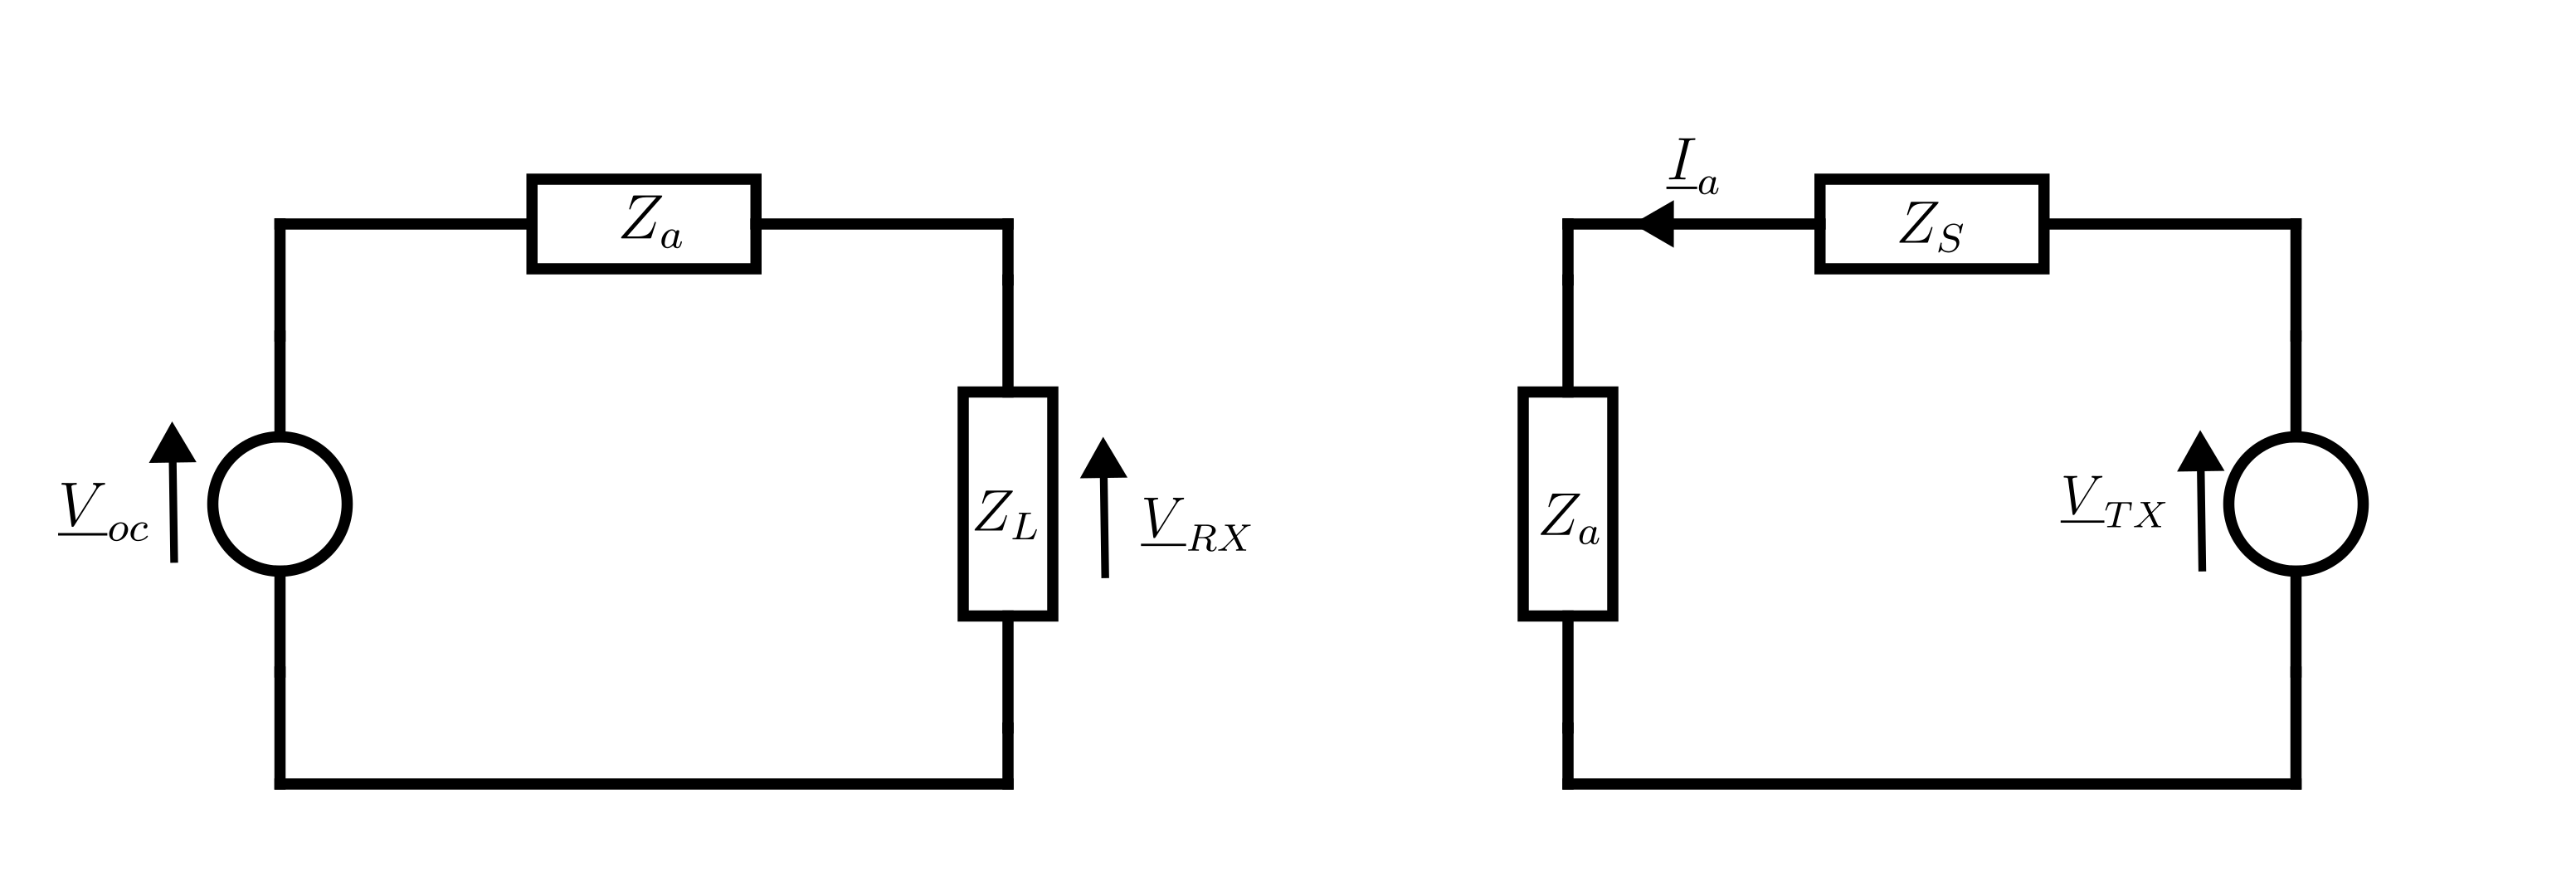
\includegraphics[width=1\textwidth]{circuit.png}
    \caption{Equivalent electric circuit of an antenna in RX (left) and TX (right)}
    \label{fig:equivalent_electrical_circuit}
\end{figure}

Fig \ref{fig:equivalent_electrical_circuit} shows the equivalent electrical circuit at RX and TX where $\underline{V}_{oc}$ is the induced voltage, $\underline{V}_{RX}$ the voltage at the output of the RX antenna, $\underline{V}_{TX}$ at the input of the TX antenna and $\underline{I}_{a}$ the current entering the TX antenna.\\

As both transmitting and receiving antenna are vertical $\lambda/2$ dipoles, their equivalent heights can be analytically computed:

\begin{align*}
    \vec{h}_e (\theta, \phi) = \frac{\lambda}{\pi} \frac{\cos(\frac{1}{2}\cos \theta)}{\sin ^2 \theta}\vec{1_z}\\
    \vec{h}_{e\perp} (\theta, \phi) = -\frac{\lambda}{\pi} \frac{\cos(\frac{\pi}{2}\cos \theta)}{\sin \theta}\vec{1_\theta}
\end{align*}

The transverse part of the equivalent height allows to give an expression for the emitted electric field.

\begin{align*}
    \underline{\vec{E}} = j\frac{Z_0\underline{I}_a}{2\pi}\frac{\cos(\frac{\pi}{2}\cos \theta)}{\sin \theta}\frac{e^{-j\beta r}}{r}\vec{1_\theta}
\end{align*}

To make the transmission parameters appear in the electric field expression, $\beta$ and $\underline{I}_a$ must be replaced using:

\begin{align*}
    \beta = \frac{2\pi f_c}{c}\\
    \underline{V}_{TX} = (Z_a + Z_S) \underline{I}_a
\end{align*}

Wich yields

\begin{align*}
    \underline{\vec{E}} = j\frac{Z_0\underline{V}_{TX}}{2\pi (Z_a + Z_S)}\frac{\cos(\frac{\pi}{2}\cos \theta)}{\sin \theta}\frac{e^{-j \frac{2\pi f_c r}{c}}}{r}\vec{1_\theta}\\
    \left . \underline{\vec{E}}\right\vert_{\theta = \pi/2} = -j\frac{Z_0\underline{V}_{TX}}{2\pi (Z_a + Z_S)}\frac{e^{-j \frac{2\pi f_c r}{c}}}{r}\vec{1_z}
\end{align*}

Where $\theta$ has been chosen equal to $\pi /2$ in order to study only the electric filed in the horizontal place. At the receiving side, the incoming electric filed $\underline{\vec{E}}_i$ is simply equal to the transmitted electric field after it traveled over a distance $r = c\tau$ where $\tau$ is the propagation delay. This is of course in the case of line of sight (LOS) communication with no interfering object (IO) between TX and RX.

\begin{align*}
    \underline{\vec{E}}_i = -j\frac{Z_0 c \underline{V}_{TX}}{2\pi (Z_a + Z_S)}\frac{e^{-j 2\pi f_c \tau}}{\tau}\vec{1_z}
\end{align*}

The voltage at the output of the antenna $\underline{V}_{RX}$ can then be deduced using:

\begin{align*}
    \underline{V}_{RX} = \frac{Z_L}{Z_a + Z_L} \underline{V}_{oc}\\
    \underline{V}_{oc} = -\left . \vec{h}_{e\perp}(\theta, \phi)\right\vert_{\theta = \pi/2} \cdot \underline{\vec{E}}_i
\end{align*}

Resulting in:

\begin{align*}
    \underline{V}_{oc} &= \frac{\lambda}{\pi} \cdot \underline{E}_i\\
    &= -j\frac{Z_0 c \lambda \underline{V}_{TX}}{2\pi^2 (Z_a + Z_S)}\frac{e^{-j 2\pi f_c \tau}}{\tau}\\
    \underline{V}_{RX} &= -j\frac{Z_0 Z_L c \lambda \underline{V}_{TX}}{2\pi^2 (Z_a + Z_L) (Z_a+Z_S)}\frac{e^{-j 2\pi f_c \tau}}{\tau}
\end{align*}

\section{Step 2}

Assuming the communication takes place via a LOS ray only, the channel impulse response $h(\tau)$ is defined as follows:

\begin{align*}
    h(\tau) = \frac{\alpha_1 e^{-j2\pi f_c \tau_1}}{d_1} \delta(\tau - \tau_1)
\end{align*}

Where $\tau_1$ is the propagation delay and $d_1$ the propagation distance of the direct ray. $\alpha_1$ (which might be complex) takes into account a phase change or attenuation due for example to reflections whereas the imaginary exponential next to it corresponds to the phase change due to the propagation delay. In the case of LOS transmission, we have $\alpha_1 = 1$.\\
The transfer function $H(f)$ of the channel is found by taking the Fourier transform of $h(\tau)$

\begin{align*}
    H(f) &= \int_{-\infty}^{\infty} h(\tau) e^{-j2\pi f \tau} d\tau\\
    &= \frac{e^{-j2\pi f_c \tau_1}}{d_1}e^{-j2\pi f \tau_1}
\end{align*}

As we consider a single ray, the narrowband model of the channel $h_{NB}$ (representing the case where the receiver perceives the sum of all propagation path) is simply found by removing the Dirac pulse from $h(\tau)$

\begin{align*}
    h_{NB} = \frac{e^{-j2\pi f_c \tau_1}}{d_1}
\end{align*}

The ratio between the received power $P_{RX}$ and the transmitted power $P_{TX}$ is found with:

\begin{align}
    \frac{P_{RX}}{P_{TX}} &= \frac{\left| h(\tau) \right|^2}{2} \nonumber\\
    &= \frac{1}{d_1^2}
    \label{eq:power_approx}
\end{align}

This result can be compared with the Friis formula, given by:

\begin{align}
    P_{RX}(d) = P_{TX} G_{TX}(\theta_{TX}, \phi_{TX})G_{RX}(\theta_{RX}, \phi_{RX})\left(\frac{\lambda}{4\pi d}\right)^2
    \label{eq:friis_formula}
\end{align}

The reason for the big difference between the two formulas can be easily explained: in eq \ref{eq:power_approx}, the powers $P_{RX}$ and $P_{TX}$ are the ones of the wave without taking the antennas into account. To correct it:

\begin{align}
    \frac{\left|\bm{\vec{\mathscr{S}}}_{RX}\right|}{\left|\bm{\vec{\mathscr{S}}}_{TX}\right|} = \frac{1}{d_1^2}
    \label{eq:poynting}
\end{align}

To compare the received and the injected power, the Poynting vectors should be replaced by

\begin{align*}
    \left|\bm{\vec{\mathscr{S}}}_{TX}\right| = G_{TX} P_{TX}\\
    \left|\bm{\vec{\mathscr{S}}}_{RX}\right| A_{eRX} = P_{RX}\\
    \text{where} \quad \quad A_{eRX} = G_{RX}\left(\frac{\lambda}{4\pi}\right)^2
\end{align*}

When placed back in eq \ref{eq:poynting}, the expression matches the Friis formula.

\begin{align}
    \frac{P_{RX}}{P_{TX}} = G_{TX} G_{RX} \left(\frac{\lambda}{4\pi d_1}\right)^2
\end{align}

Two deductions can be made of this result: 
\begin{itemize}
    \item The power loss on the channel depends on the square of the distance between the emitter and the receiver. It implies that doubling the range of an antenna would a multiplication of the transmitting power by a factor 4.
    \item A more surprising result is the wavelength squared appearing at the numerator. It shows that there is always a compromise between data rate and power consumption as a larger wavelength will indeed be less attenuated but the maximal data rate will then be lowered in order for the bandwidth of the transmitted signal to be much lower than the carrier frequency.
\end{itemize}

\section{Step 3}




%\printglossary

%\printglossary[type=\acronymtype]

%Bibliography
%\nocite{*}
%\printbibliography[type=article,title=Articles]

\end{document}	
